\chapter{Experimentelle Details} \label{chapter:exp_details}

Im Folgenden sollen die in dieser Arbeit verwendeten Aufbauten und Methoden für das experimentelle Gewinnen von Daten vorgestellt werden. Dies beinhaltet NMR-Apparaturen wie Spektrometer und Probenköpfe, die Weiterverarbeitung der Daten, sowie die untersuchten Proben und deren Herstellung.

\section{Spektrometer} \label{section:exp:spektrometer}

Für diese Arbeit wurden zwei Spektrometer verwendet: Zum einen ein kommerziell erhältliches Spektrometer der Firma Bruker, welches mit einem Magneten mit einer Protonenfrequenz von etwa $\SI{400}{MHz}$ operiert; zum anderen ein Eigenbau, intern „OBI“ genannt, welcher eine Protonenfrequenz von etwa $\SI{300}{MHz}$ hat. Beide sind in Abbildung \ref{fig:exp:proben} dargestellt.

Der Aufbau des OBI-Spektrometers ist in Abbildung \ref{fig:exp:aufbau} skizziert und soll im Folgenden vorgestellt werden. Die Weiterverarbeitung der mit dem Spektrometer gewonnenen Daten, sowie die Temperaturkontrolle (die, ebenso wie der supraleitende Magnet in der Abbildung nicht gezeigt ist), werden danach besprochen.

\begin{figure}
	\centering
	\begin{subfigure}{.35\textwidth}
		\centering
		\includegraphics[width=0.95\textwidth]{graphics/spektrometer/IMG_43372.JPG}
		\caption{ }
		\label{fig:exp:OBI}
	\end{subfigure}%
	\begin{subfigure}{.35\textwidth}
		\centering
		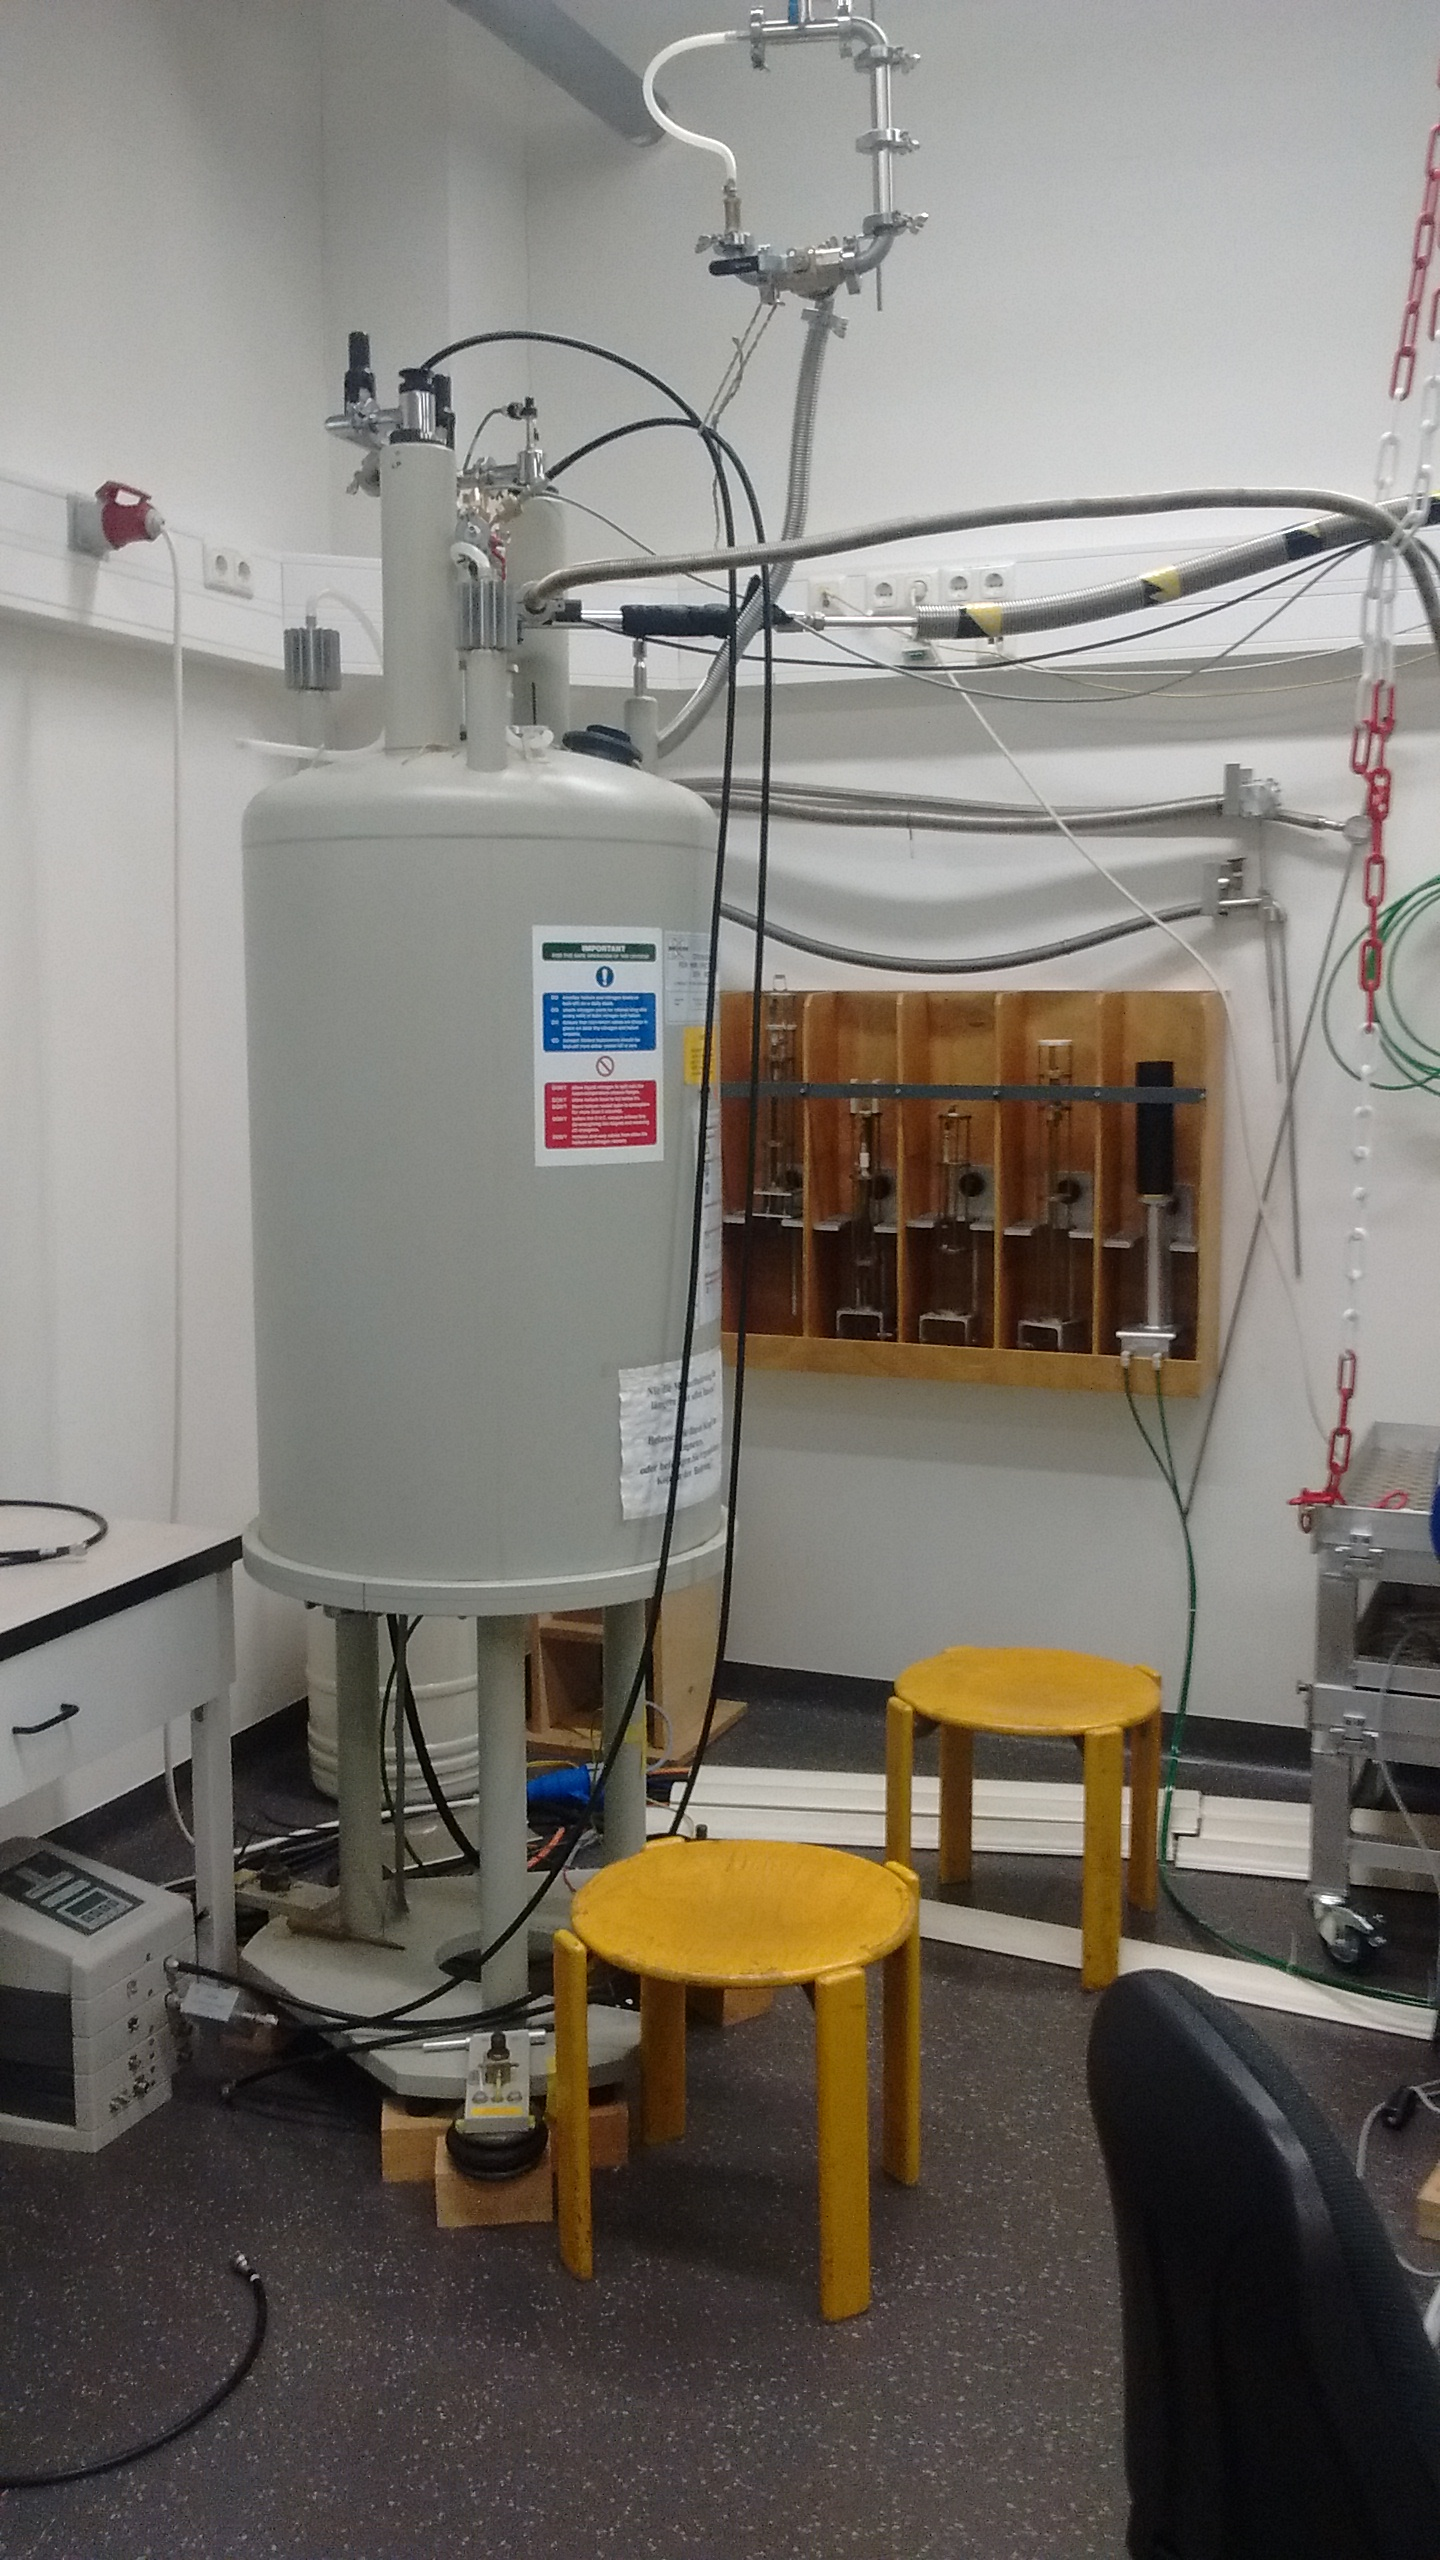
\includegraphics[width=0.95\textwidth]{graphics/spektrometer/IMG_20180419_160711175.jpg}
		\caption{ }
		\label{fig:exp:bruker}
	\end{subfigure}
	\caption{Fotografien der verwendeten Spektrometer. Links das OBI-Spektrometer, rechts das Bruker-Spektrometer.}
	\label{fig:exp:proben}
\end{figure}

\begin{figure}
	\begin{center}
		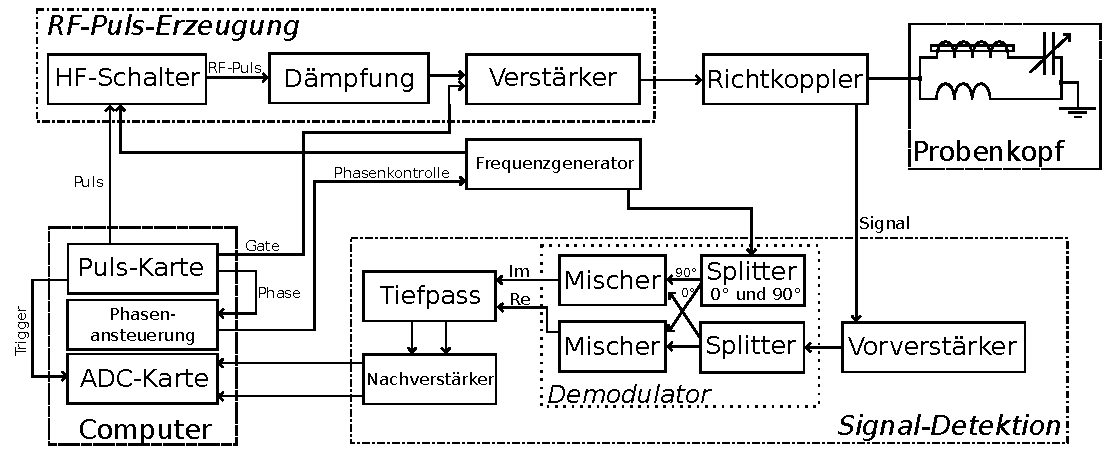
\includegraphics[width=\textwidth]{graphics/joachim/aufbau.pdf} 
	\end{center}
	\caption{Skizzierter Aufbau eines NMR-Spektrometers. Abbildung aus \cite[S. 29]{lueg_implementierung_2016}} \label{fig:exp:aufbau}
\end{figure}

Die Beschreibung vollzieht den Aufbau entlang des Signalwegs nach. Die Steuerung aller Messungen geschieht über einen Computer, der mit der in Python geschriebenen Software DAMARIS (Darmstadt Magnetic Resonance Instrument Software \cite{gadke_damaris_2007}) ausgestattet ist. Diese erlaubt es, Messprogramme zu definieren, mit Hilfe von Pythons serieller Schnittstelle die Verbindung zu verschiedenen Geräten herzustellen, und die produzierten Signale aufzunehmen, anzuzeigen und zur Weiterverarbeitung zu speichern.

Durchgängig läuft ein Frequenzgenerator, dessen Frequenz auf die Larmorfrequenz des zu untersuchenden Kerns im jeweiligen Magneten eingestellt ist. Ist diese Frequenz nicht bekannt, empfiehlt sich in der Regel das Aufnehmen eines Spektrums von einer Flüssigkeit oder Lösung, die den gewünschten Kern enthält. Aufgrund der geringen Breite des Flüssigkeitsspektrum lässt sich so die magnetfeldabhängige Larmorfrequenz bestimmen.

Soll ein Puls an den Probenkopf gesandt werden, setzt DAMARIS über eine 24-bit-Puls-Karte für die Dauer des Pulses ein Bit auf 1, was mit Hilfe eines HF-Schalters aus dem kontinuierlichen Signal des Frequenzgenerators einen Puls mit der gewünschten Länge ausschneidet.

Dieser Puls wird nun gedämpft. Über diese variable Dämpfung lässt sich die Stärke des Pulses und damit aufgrund der Beziehung $B_\text{Spule} \propto I_\text{Puls}$ das in der Probenspule entstehende Magnetfeld variieren. Dieses wiederum ist nach Formel \eqref{eqn:theo:pulslaenge} entscheidend für die Länge aller Pulse. Es sollte die Dämpfung so eingestellt werden, dass sich die Länge eines $\SI{180}{\degree}$-Invertierungspulses im Bereich weniger Mikrosekunden befindet.

Der so gedämpfte Puls wird dann mit einem Verstärker um einen konstanten Faktor verstärkt und trifft dann über einen Richtkoppler auf den Probenkopf. Das nach dem Puls vom Probenkopf zurückgegebene Signal wird vom Richtkoppler zur Signal-Detektion geleitet. Es wird zunächst von einem Vorverstärker verstärkt, ehe es gesplittet wird. Beide Teile werden mit der vom Frequenzgenerator erzeugten Sinus-Schwingung, welche die Larmorfrequenz hat, gemischt; eine der Schwingungen ist jedoch um $\SI{90}{^\circ}$ phasenverschoben. Die so entstehenden Signale werden Real- und Imaginärteil des Signals genannt. Zusätzlich können beide Teile um eine konstante Phase verschoben werden. Diese lässt sich wiederum über DAMARIS mit einer Phasenansteuerungs-Karte einstellen.

Im nachfolgenden Tiefpass werden alle hochfrequenten Teile des Signals abgeschnitten, sodass nur die durch das Mischen entstandende Differenz $\Delta \omega = \omega_L - \omega_\text{Signal}$ verbleibt. Es lässt sich die Cutoff-Frequenz sowie die Amplitude und der Offset beider Einzelsignale einstellen. Die letzteren Beiden sollten so gewählt sein, dass der Offset Null ist und beide Signale die gleiche Amplitude haben.


Beide Signale werden mit einem Nachverstärker verstärkt, ehe sie von einer ADC-Karte (engl. ADC: Analog-Digital-Konverter) des Computers in Form von Amp\-li\-tu\-den-Wer\-ten in der gesetzten Frequenz von bis zu $\SI{10}{MHz}$ aufgenommen werden. Die ADC-Karte wird dabei über die Puls-Karte mit einem Trigger geschaltet. Dies kann notwendig sein, da vor dem eigentlichen Signal noch unerwünschte Effekte, wie zum Beispiel ein Nachschwingen der Probenspule, auftreten können. Um diese abzuschneiden, kann das Aufnehmen des Signals um eine festgelegte Trigger-Zeit verzögert werden.

Für mehr Informationen zu den hier beschriebenen Aufbauten können \cite{lueg_implementierung_2016} und \cite{tilly_master} herangezogen werden.



\section{Weiterverarbeitung der Signale} \label{section:exp:weiterverarbeitung}

Alle so aufgenommen Daten bestehen aus einem Zeitpunkt $t$ und dem zugehörigen Amplitudenwert von Real- und Imaginärteil. Werden Messungen wie eine $T_1$-, $T_2$- oder $F_2$-Messung durchgeführt, ergeben sich variablenabhängige Messreihen. Es wird diese Variable (z.B. Evolutions- oder Mischzeit) meist logarithmisch gegen das Maximum des Realteils der jeweiligen Messung aufgetragen; dann können die Daten analysiert werden. Um ein möglichst großes Realteil-Signal am Ort $t_\text{Max}$ des Maximums zu gewährleisten, sollte dort der Imaginärteil einen Nulldurchgang aufweisen. Dies lässt sich mit einer entsprechenden Einstellung der Phase über die Phasenansteuerungs-Karte erreichen.

Sollen Spektren untersucht werden, wird das Zeitsignal fouriertransformiert. Für eine hohe Auflösung sollte ein möglichst langes Zeitsignal aufgenommen werden; für eine große Frequenz-Spanne ein Zeitsignal mit möglichst hoher Frequenz der ADC-Karte.



\section{Probenköpfe} \label{section:exp:probenkoepfe}

NMR-Messungen bei mehreren Hundert Grad Celsius durchzuführen, kann sich mitunter als eine Herausforderung gestalten. Lötzinne, die häufig verwendet werden um die Resonanzspule an dem Probenkopf anzubringen, schmelzen je nach Art bei weniger als $\SI{200}{\degreeCelsius}$. Aber auch Tuningkondensator und Match\-ing\-spu\-le sowie der für die Resonanzspule verwendete Draht sind häufig nur für bestimmte Temperaturen ausgelegt. Zudem ist es offensichtlich, dass für höhere Temperaturen eine gute Isolierung und gegebenenfalls Kühlung des Probenkopfs gegeben sein muss, befindet er doch in direkter Umgebung des mit flüssigem Helium gekühlten Magneten.

Für solche Anwendungen ist also ein spezieller Probenkopf notwendig, welcher in Form des Hochtemperaturprobenkopfs (intern als „Ofen“ bezeichnet) als eine Spezialanfertigung realisiert wurde. Dessen Konstruktionszeichnung ist in Abbildung \ref{fig:exp:ofen_aufbau} zu sehen; eine detaillierte Beschreibung findet sich in \cite{tilly_master}.

\begin{sidewaysfigure}
	\begin{figure}[H]
		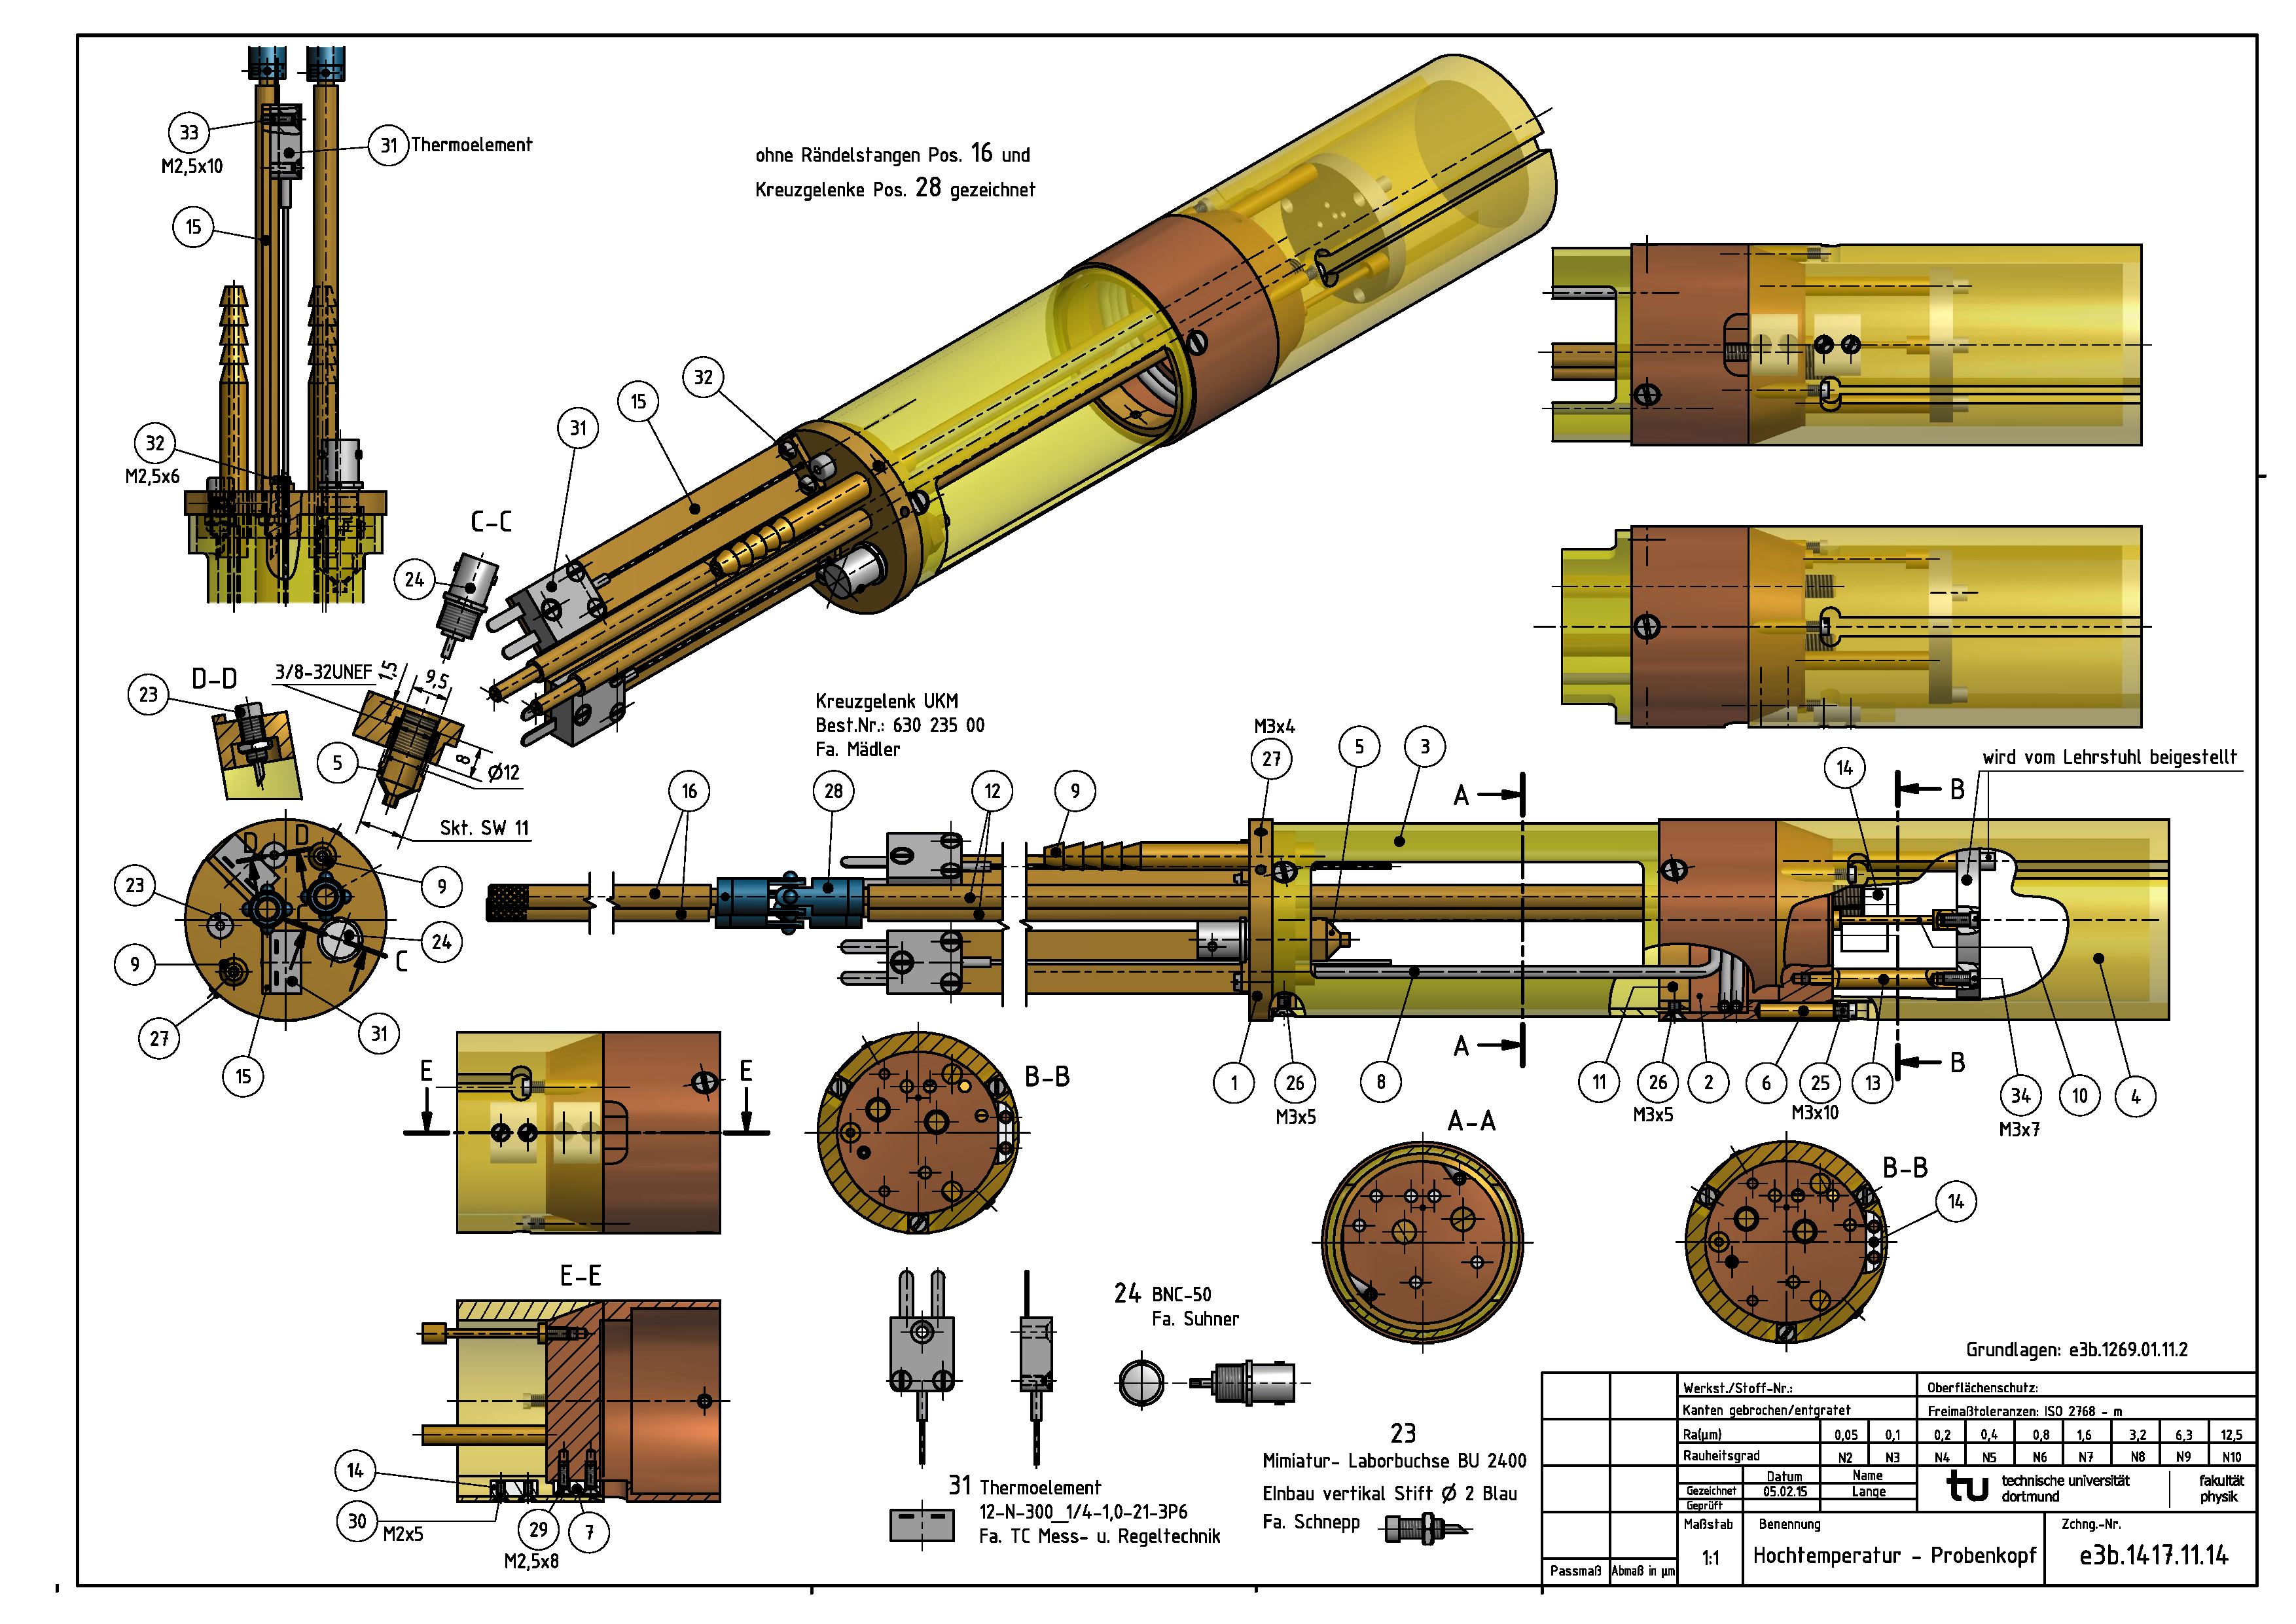
\includegraphics[width=1.05\textheight]{graphics/ofen/ofen_aufbau2.pdf}
		\caption{Konstruktionszeichnung des Hochtemperaturprobenkopfes \cite{Rudloff_blue_print}.}
		\label{fig:exp:ofen_aufbau}
	\end{figure}
\end{sidewaysfigure}

Er lässt sich grob in drei Teilen beschreiben: Im oberen Drittel befindet sich der Schwingkreis mit der Probe, eine Vorrichtung, um diese zu erwärmen, sowie die dazugehörige notwendige thermische Isolation. Am unteren Drittel werden alle notwendigen Verbindungen angeschlossen; das mittlere Drittel verbindet beides und beherbergt einen Netzfilter.

Um Temperaturen von bis zu $\SI{1100}{K}$ erreichen zu können, wird ein Heizdraht aus einer FeCrAl-Legierung verwendet. Dieser ist bifilar über einen Hartkeramik-Hohlzylinder gewickelt, um möglichst wenig störende Magnetfelder entstehen zu lassen -- gerade in direkter Umgebung der Probe. Diese Vorrichtung ist im Deckel untergebracht, der sich über die aus Platin bestehende Probenspule stülpen lässt.

Um die entstehende Hitze möglichst gut nach außen hin zu isolieren, ist dieser Aufbau von poröser Keramik umgeben -- sowohl innerhalb des Deckels als auch zwischen Probenspule und Rest des Probenkopfes. Bei letzterem ist zudem eine weitere Scheibe aus dichter Keramik vorhanden. Für die Probenspule und Temperaturfühler sind Bohrungen in den Keramikscheiben vorhanden, über die sie mit dem Rest des Probenkopfes verbunden werden können.

Darunter befindet sich der Schwingkreis der Probenspule. Sowohl eine Match\-ing\-spu\-le als auch ein variabler Kondensator und eine Halterung für einen wechselbaren Kondensator sind vorhanden. Es lassen sich Kondensatoren mit verschiedenen Kapazitäten in der Halterung anbringen; zusammen mit dem variablen Kondensator kann so für die Resonanzfrequenz eine Spanne von $\SI{63,6}{MHz}$ bis $\SI{168,9}{MHz}$ (mit Unterbrechungen) abgedeckt werden. Darunter befindet sich die Möglichkeit für eine Wasserkühlung.

Der sich in dem Verbindungsteil befindliche Netzfilter soll den Heizstrom von störenden Anteilen befreien. Dazu wird eine Spule mit eisernem Kern verwendet. Während diese Drossel den Probenkopf in der Vergangenheit genau im Hauptfeld des Magneten gehalten hatte, ist dies jetzt nicht mehr der Fall, was eine Messung sehr schwer macht. Da zudem inhomogenes Gesamtmagnetfeld am Ort der Probe durch das zusätzliche Magnetfeld zu befürchten sind, liegt die Idee nahe, den vorliegenden Aufbau zu ändern. Eine mögliche Anpassung könnte sein, den Netzfilter außerhalb des Probenkopfes anzubringen und die Positionierung des Probenkopfes im Hauptfeld des Magneten durch eine zusätzliche Halterung zu gewährleisten.

Um den Aufbau zu betreiben, sind im unteren Drittel eine Reihe von Anschlüssen vorhanden:
\begin{itemize}
	\item Ein BNC-Anschluss der vom Richtkoppler kommend zum Schwingkreis führt,
	\item Bohrungen für die beiden Thermoelemente, welche von einem Temperatur-Controller ausgelesen werden,
	\item ein Anschluss für den Heizstrom, welcher von einem Temperatur-Controller bereitgestellt wird,
	\item je eine Rändelstange für die Einstellung von Matching\-spu\-le und Tuningkondensator,
	\item Anschlüsse für Zu- und Abflussschläuche für das Kühlwasser. Der Zufluss kann mit einem Wasserhahn reguliert werden.
\end{itemize}

Unter anderem aufgrund der beschriebenen Probleme mit der Positionierung des Hochtemperaturprobenkopfes im Magnetfeld war dieser Probenkopf nicht einsatzfähig um die im Rahmen dieser Arbeit geplanten Messungen durchzuführen. Daher wurde der Probenkopf für keine der im Verlauf der Arbeit präsentierten Messungen verwendet.

„Reguläre“ Probenköpfe sind im Vergleich zum Hochtemperaturprobenkopf recht einfach gehalten. Da die Temperatursteuerung meist nicht durch den Probenkopf selbst geleistet wird, fallen die Heizeinheit, Isolation, Wasserkühlung und Netzfilter heraus, und es bleiben nur Schwingkreis und Temperaturfühler. Dies ist zum Beispiel bei dem, mit dem OBI-Spektrometer verwendeten, Probenkopf P1 der Fall. Dieser besitzt zudem keine Match\-ing\-spu\-le, sodass sich das Abstimmen des Probenkopfs deutlich umständlicher gestaltet und durch eine sehr genaue (und dadurch aufwändigere) Wickelung der Probenspule geleistet werden muss.

Das Bruker-Spektrometer verwendet einen zum Spektrometer gehörigen, kommerziellen Probenkopf. Beide Probenköpfe sind in Abbildung \ref{fig:exp:probenkoepfe} dargestellt.
\begin{figure}
	\centering
	\begin{subfigure}{.35\textwidth}
		\centering
		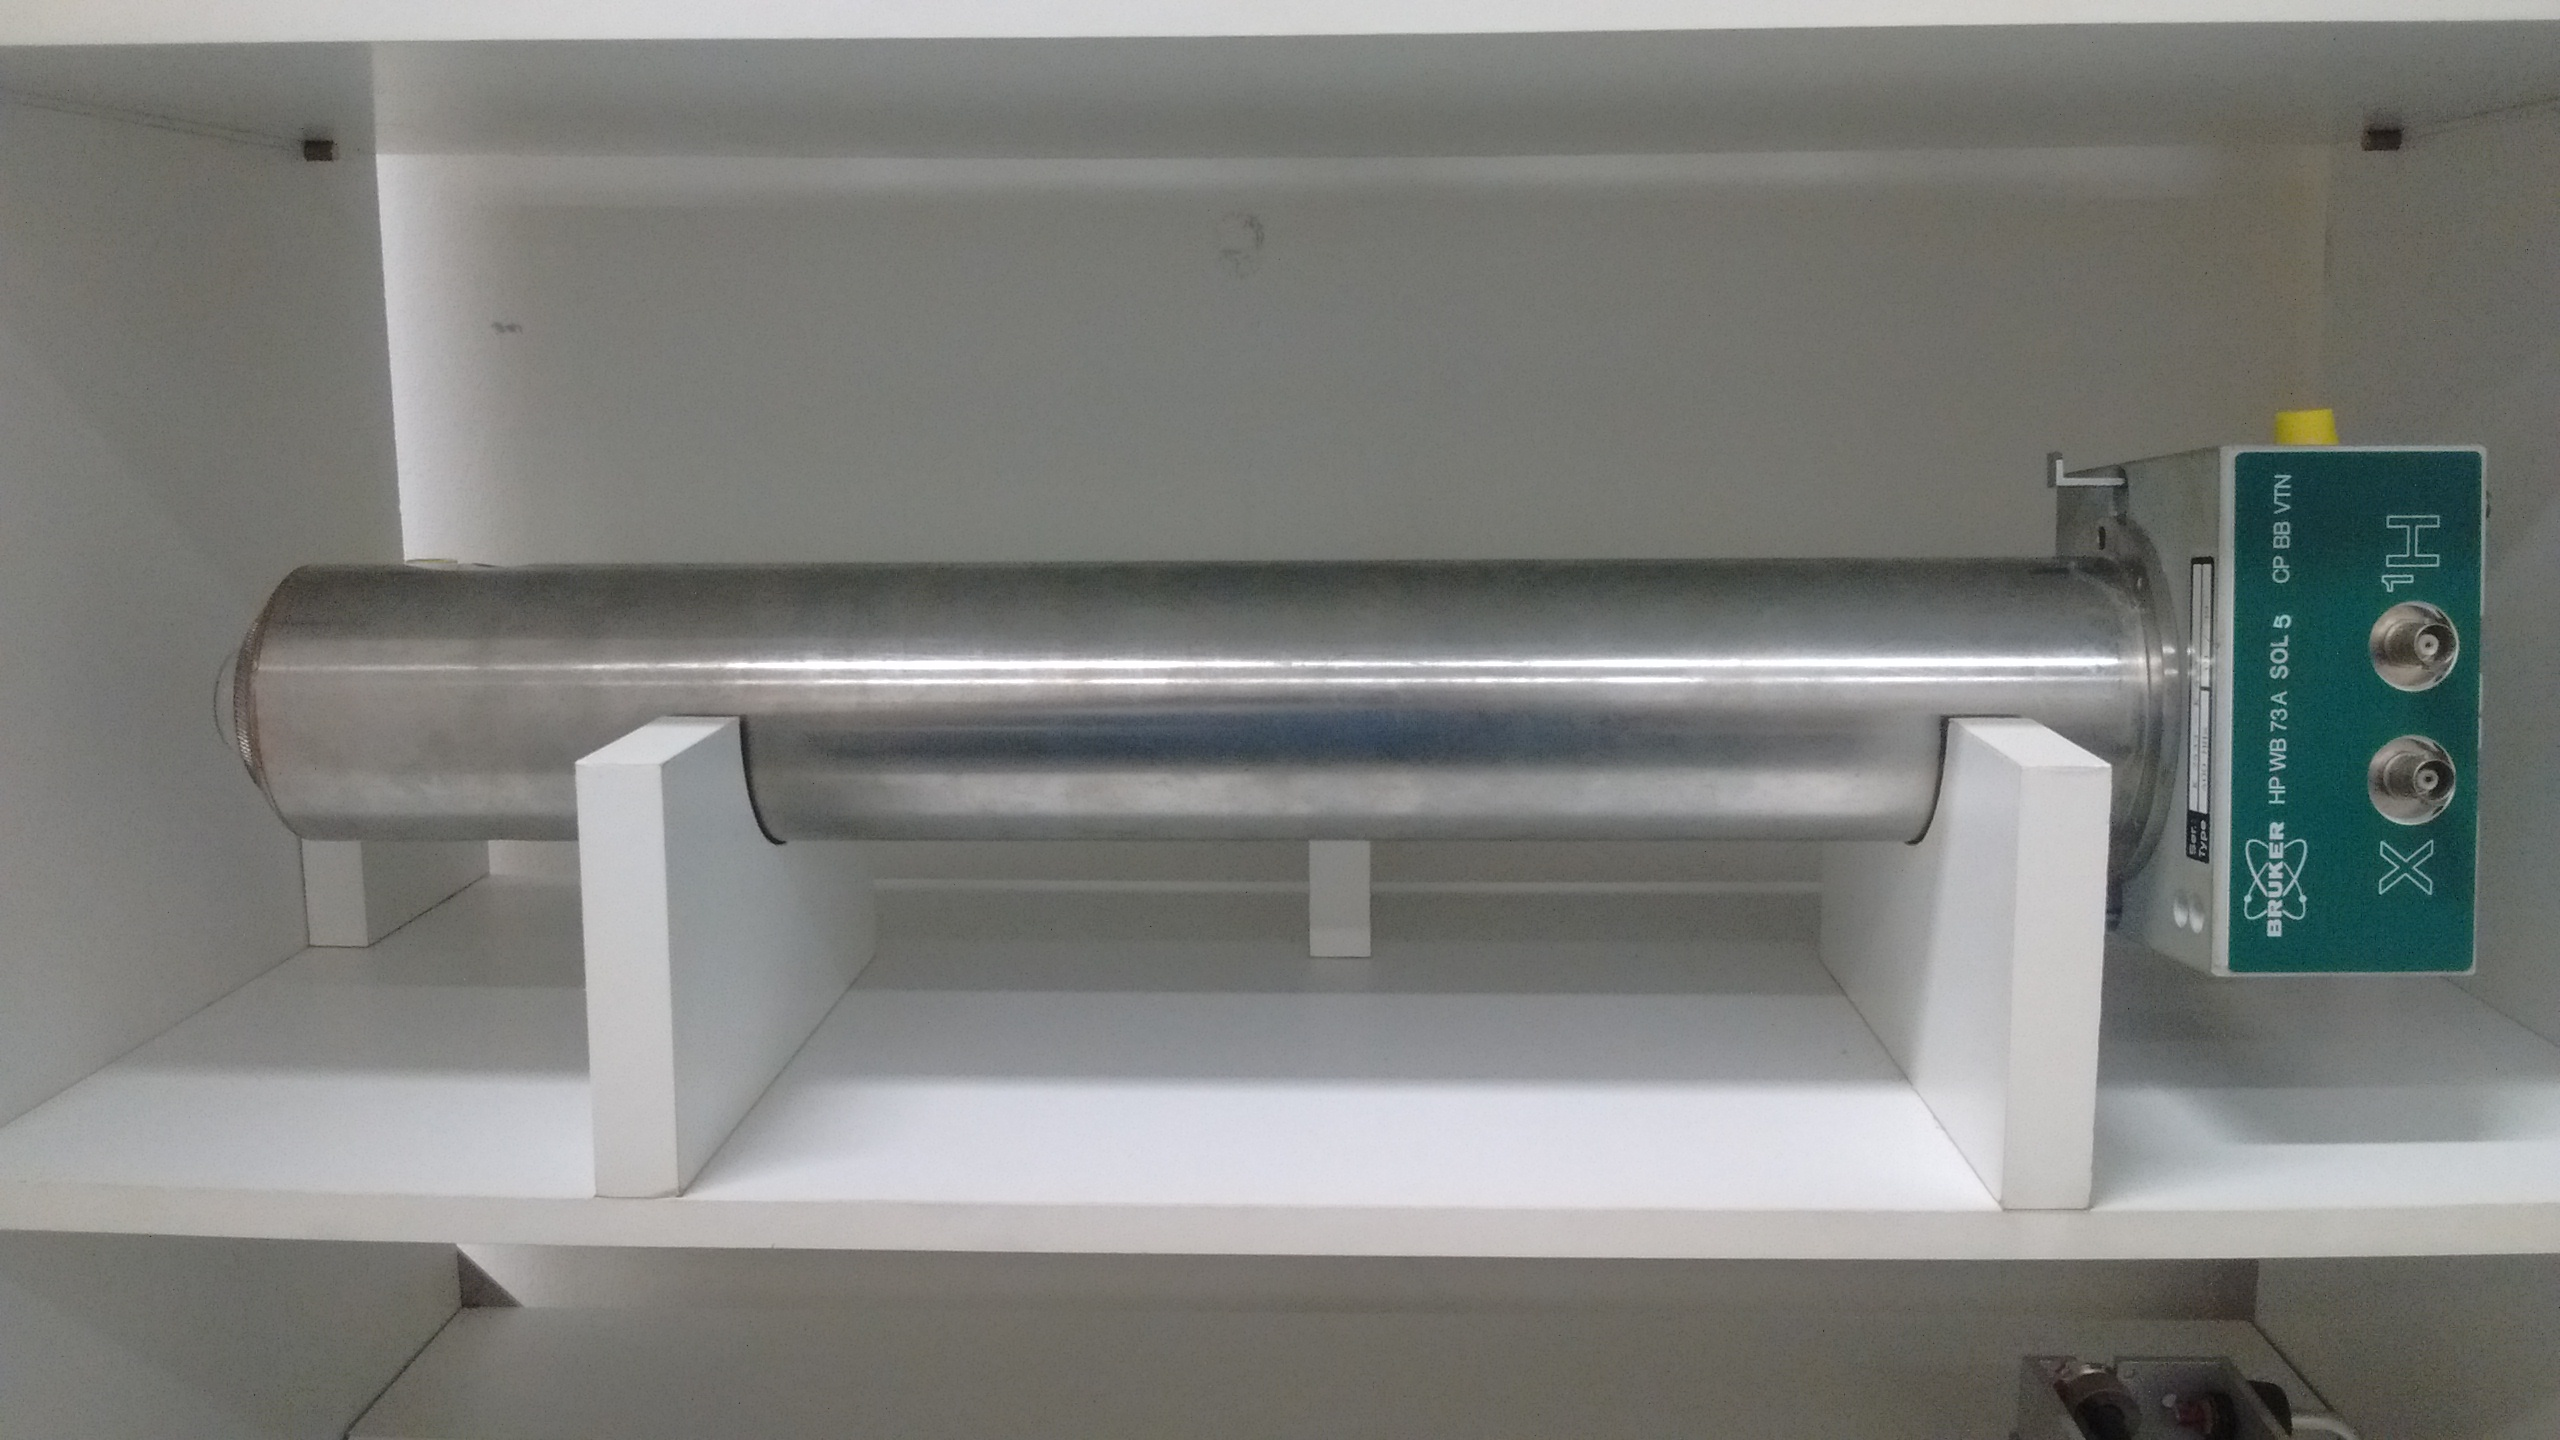
\includegraphics[width=0.95\textwidth]{graphics/probenkopf/IMG_20180419_160830226.jpg}
		\caption{ }
		\label{fig:exp:probenkopf_bruker}
	\end{subfigure}%
	\begin{subfigure}{.10\textwidth}
		\centering
		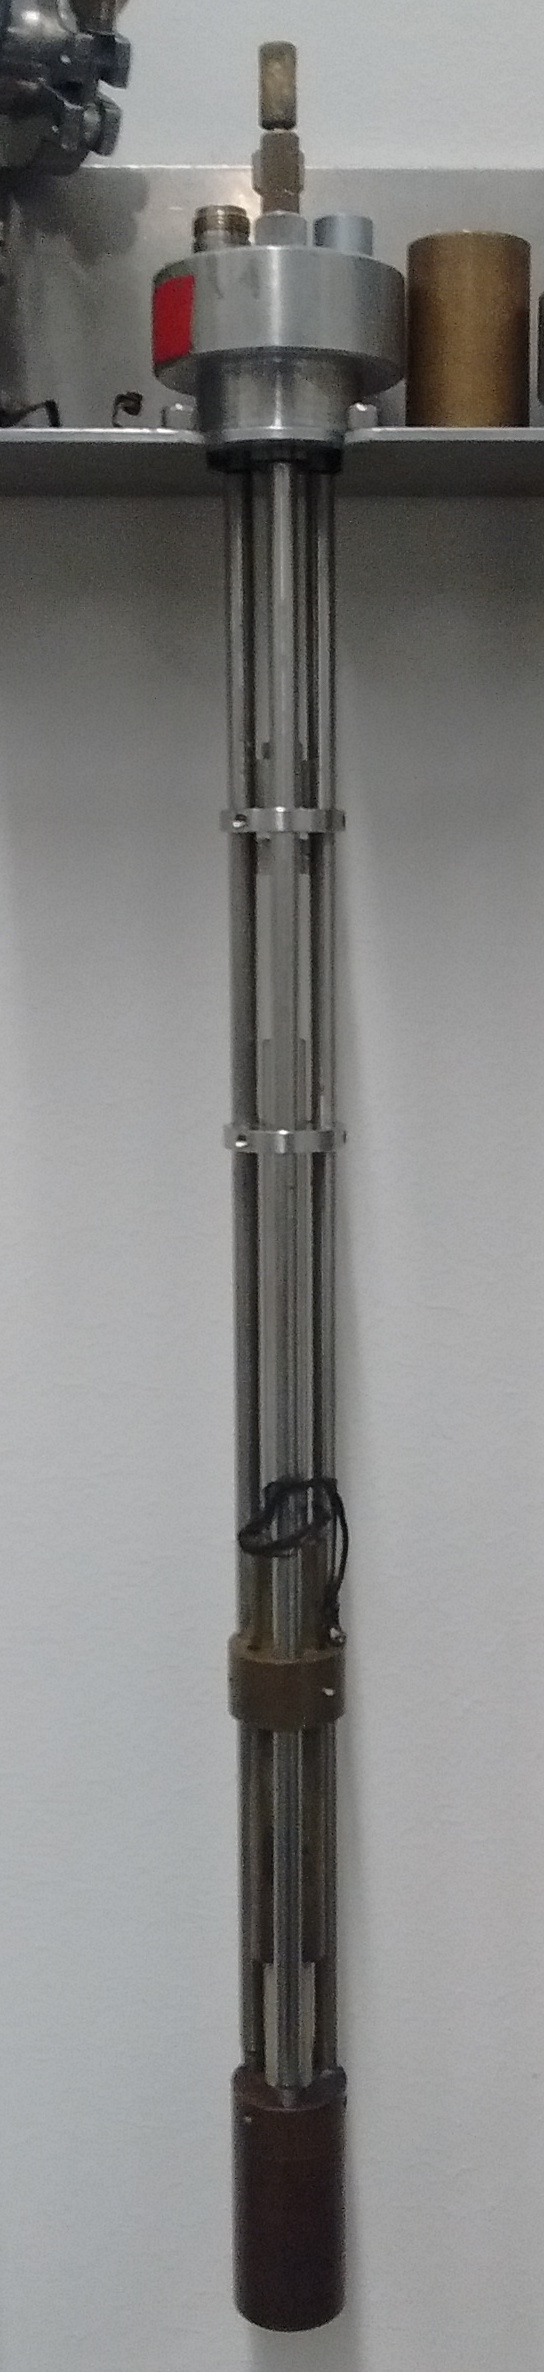
\includegraphics[width=0.95\textwidth]{graphics/probenkopf/probenkopf_p1.jpg}
		\caption{ }
		\label{fig:exp:probenkopf_obi}
	\end{subfigure}
	\caption{Fotografien der verwendeten Probenköpfe. Links der Probenkopf des Bruker-Spektrometers, rechts der Probenkopf des OBI-Spektrometers mit der Kennzeichnung P1.}
	\label{fig:exp:probenkoepfe}
\end{figure}



\section{Temperaturkontrolle} \label{section:exp:temperaturkontrolle}

Um häufig gewünschte temperaturabhängige Messungen durchführen zu können, lassen sich über Pythons serielle Schnittstelle Temperatur-Controller, wie zum Beispiel die beim OBI-Spektrometer verwendeten Lakeshore-Einheiten, benutzen. So wird ein Auslesen der aktuellen Temperatur sowie das Setzen einer Soll-Temperatur ermöglicht. Der Temperatur-Controller wiederum steuert Temperatureinheiten im Probenkopf (im Falle des Hochtemperaturprobenkopfs) oder im Kryostaten (im Falle des Probenkopfs P1) an. Die aktuelle Temperatur wird über Temperaturfühler erfasst. Dabei handelt es sich im Falle des Hochtemperaturprobenkopfes um Thermoelemente vom Typ N, im Falle des Probenkopfes P1 um PT100-Elemente.

Im Bruker-Probenkopf kann die Probe durch einen erwärmten Luftstrom, der zur Probe geleitet wird, auf bis zu $\SI{390}{\kelvin}$ erwärmt werden. 

Das OBI-Spektrometer hat zudem die Option, die Probe abzukühlen. Dazu wird, mit Hilfe eines Unterdrucks, aus einer Kanne mit flüssigem Stickstoff kaltes Stickstoffgas an der Probe vorbei geleitet. Da das Kühlen auf diese Weise nicht sehr präzise ist, kann mit dem Kryostaten gegengeheizt werden, um die gewünschte Temperatur zu erreichen. Auf diese Weise kann das OBI-Spektrometer Temperaturen von etwa $\SI{80}{\kelvin}$ bis $\SI{440}{\kelvin}$ abdecken.




\section{Proben} \label{section:exp:proben}

% \section{Der Glasbildner CRN} \label{section:theo:crn}

CRN, kurz für Calciumrubidiumnitrat, ist eine Mischung aus Calciumnitrat und Rubidiumnitrat. Der Schmelzpunkt hat bei einem Mischungsverhältnis von $2 : 3$ ein Minimum. Dieses Mischungsverhältnis liegt bei dem in dieser Arbeit verwendeten Stoff vor; dessen Summenformel lautet dementsprechend $[\text{Ca}(\text{NO}_\text{3})_\text{2}]_\text{2}[\text{RbNO}_\text{3}]_\text{3}$. Wird die Substand von einem geschmolzenen Zustand schnell genug abgekühlt, bildet sich ein Glas, dessen Glasübergangstemperatur bei $\SI{333}{K}$ liegt \cite{PIMENOV199793}. In der Umgebung dieses Punktes wurde ein Großteil der Messungen durchgeführt.

Es wurde an $^\text{87}$Rb gemessen, welches aufgrund seines höheren gyromagnetischen Verhältnisses von $\gamma = 2\pi \cdot \SI{13.984}{Mhz / T}$, trotz eines verhältnismäßig geringem natürlichen Vorkommen von $\SI{27.83}{\percent}$ dem häufigeren Isotop $^\text{85}$Rb für NMR-Untersuchungen vorzuziehen ist. $^\text{87}$Rb hat einen Kernspin von $\sfrac{3}{2}$ und ein Quadrupolmoment von $\SI{133.5}{mb}$.

Bei den durchgeführten Messungen wurden sechs verschiedene Proben verwendet:

\begin{table}[H]
	\centering
	\begin{tabular}{rllllllrl}
		\hline
		ID & Chemikalie & Hersteller & Datum & Glas & Form & \diameter & Foto \\ 
		\hline
		1	& CRN &	C. Zürn &	16.04.97 &	? &	gebogen & 	$\SI{6}{\milli\meter}$ &	(a) \\
2	& CRN &	J. Adam &	13.07.17 &	Duran &	gebogen & 	$\SI{6}{\milli\meter}$ &	(b) \\
3	& CRN &	J. Adam &	30.08.17 &	Duran &	gerade & 	$\SI{5}{\milli\meter}$ &	(c) \\
4	& CRN &	J. Adam &	30.08.17 &	Duran &	gebogen & 	$\SI{5}{\milli\meter}$ &	--- \\
5	& RbCl in D$_\text{2}$O &	J. Adam &	30.08.17 &	Duran &	gerade & 	$\SI{5}{\milli\meter}$ &	(d) \\
6	& RbCl in D$_\text{2}$O &	J. Adam &	30.08.17 &	Duran &	gebogen & 	$\SI{5}{\milli\meter}$ &	(d) \\ \hline
	\end{tabular} 
	\caption{In dieser Arbeit verwendete Proben. CRN bezeichnet dabei 2Ca(NO$_\text{3}$)$_\text{2}$-3RbNO$_\text{3}$. \label{tab:exp:proben}}
\end{table}

\begin{figure}[H]
	\centering
	\begin{subfigure}{.24\textwidth}
		\centering
		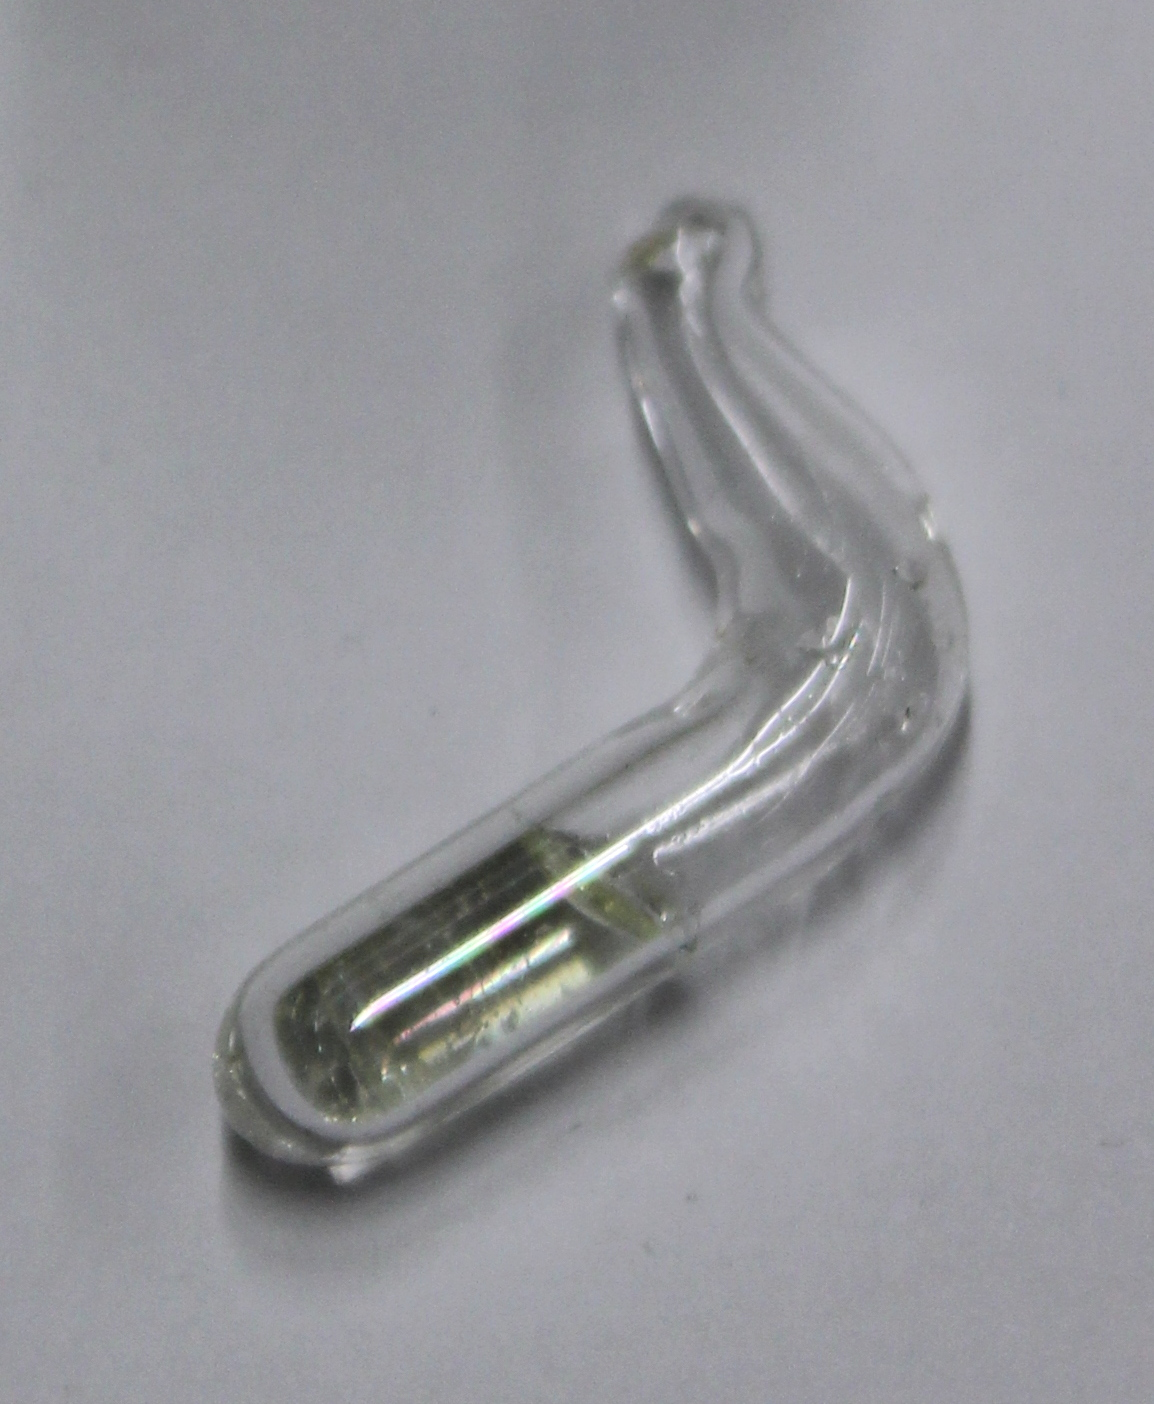
\includegraphics[width=0.95\textwidth]{graphics/proben/CRN_zuern.jpg}
		\caption{ }
		\label{fig:exp:probe_a}
	\end{subfigure}%
	\begin{subfigure}{.24\textwidth}
		\centering
		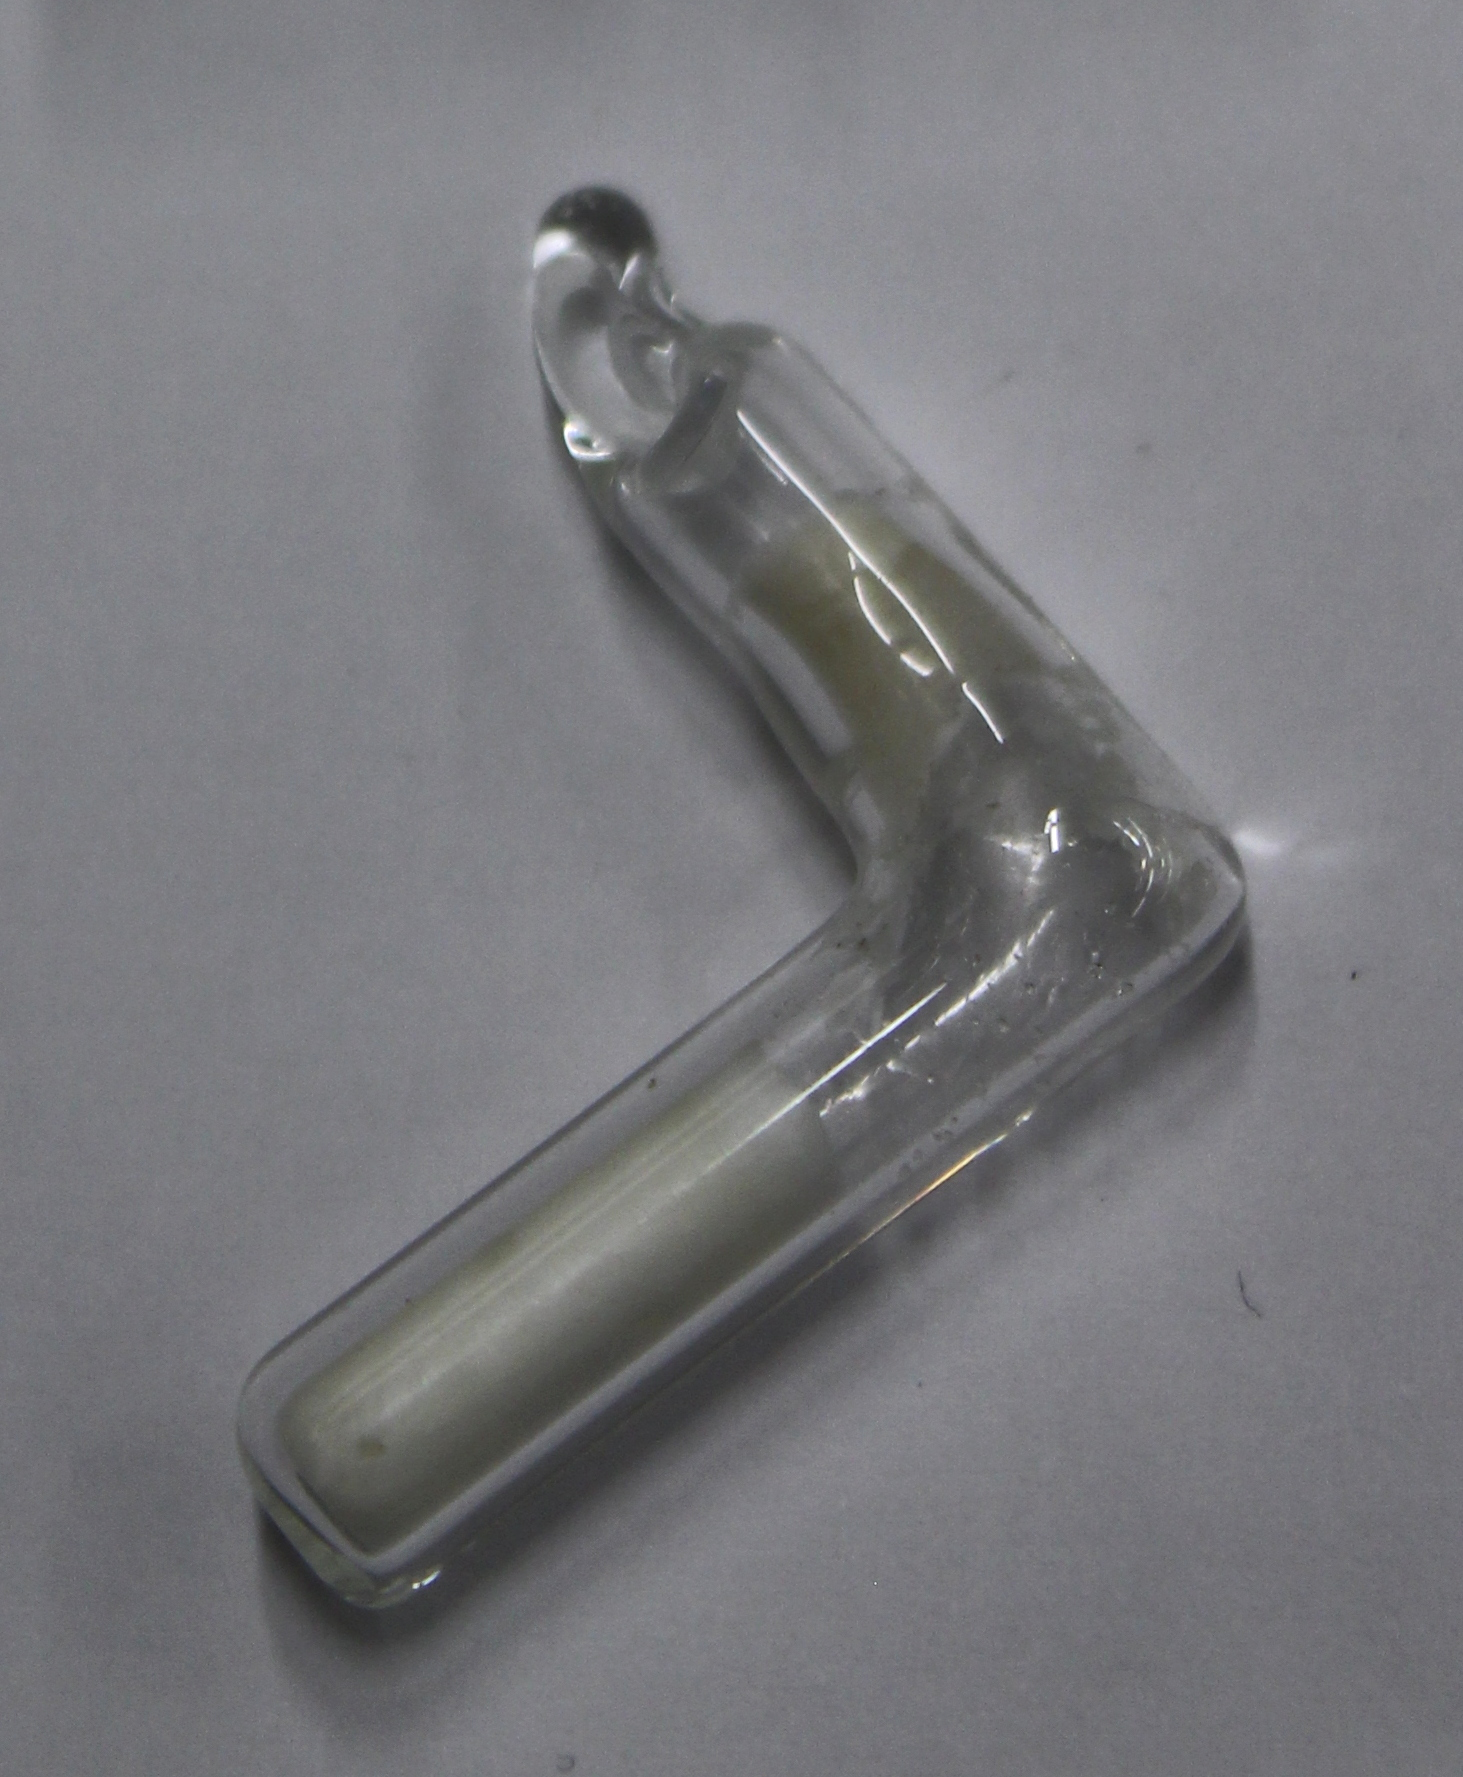
\includegraphics[width=0.95\textwidth]{graphics/proben/CRN_alt.jpg}
		\caption{ }
		\label{fig:exp:probe_b}
	\end{subfigure}
	\begin{subfigure}{.24\textwidth}
		\centering
		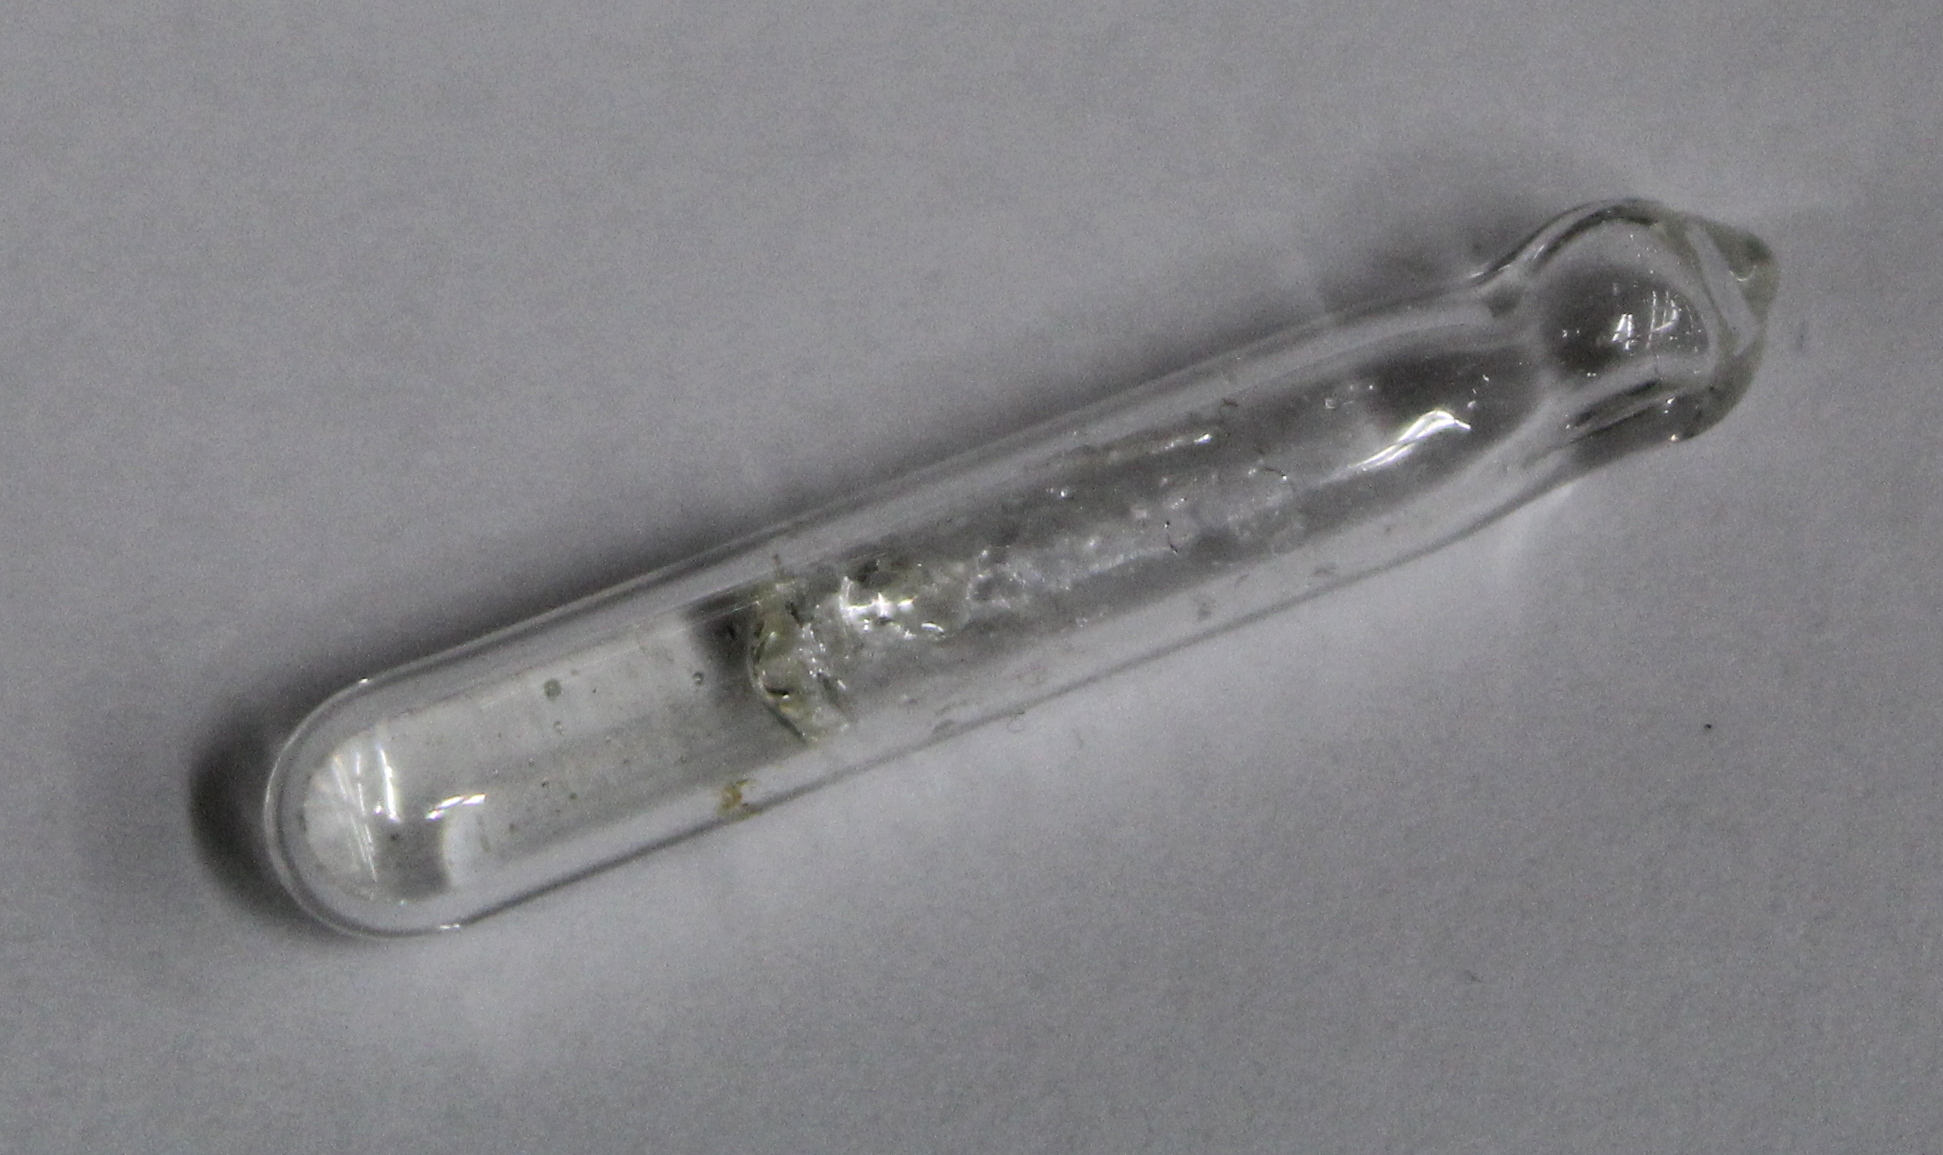
\includegraphics[width=\textwidth]{graphics/proben/CRN_neu.jpg}
		\caption{ }
		\label{fig:exp:probe_c}
	\end{subfigure}
	\begin{subfigure}{.24\textwidth}
		\centering
		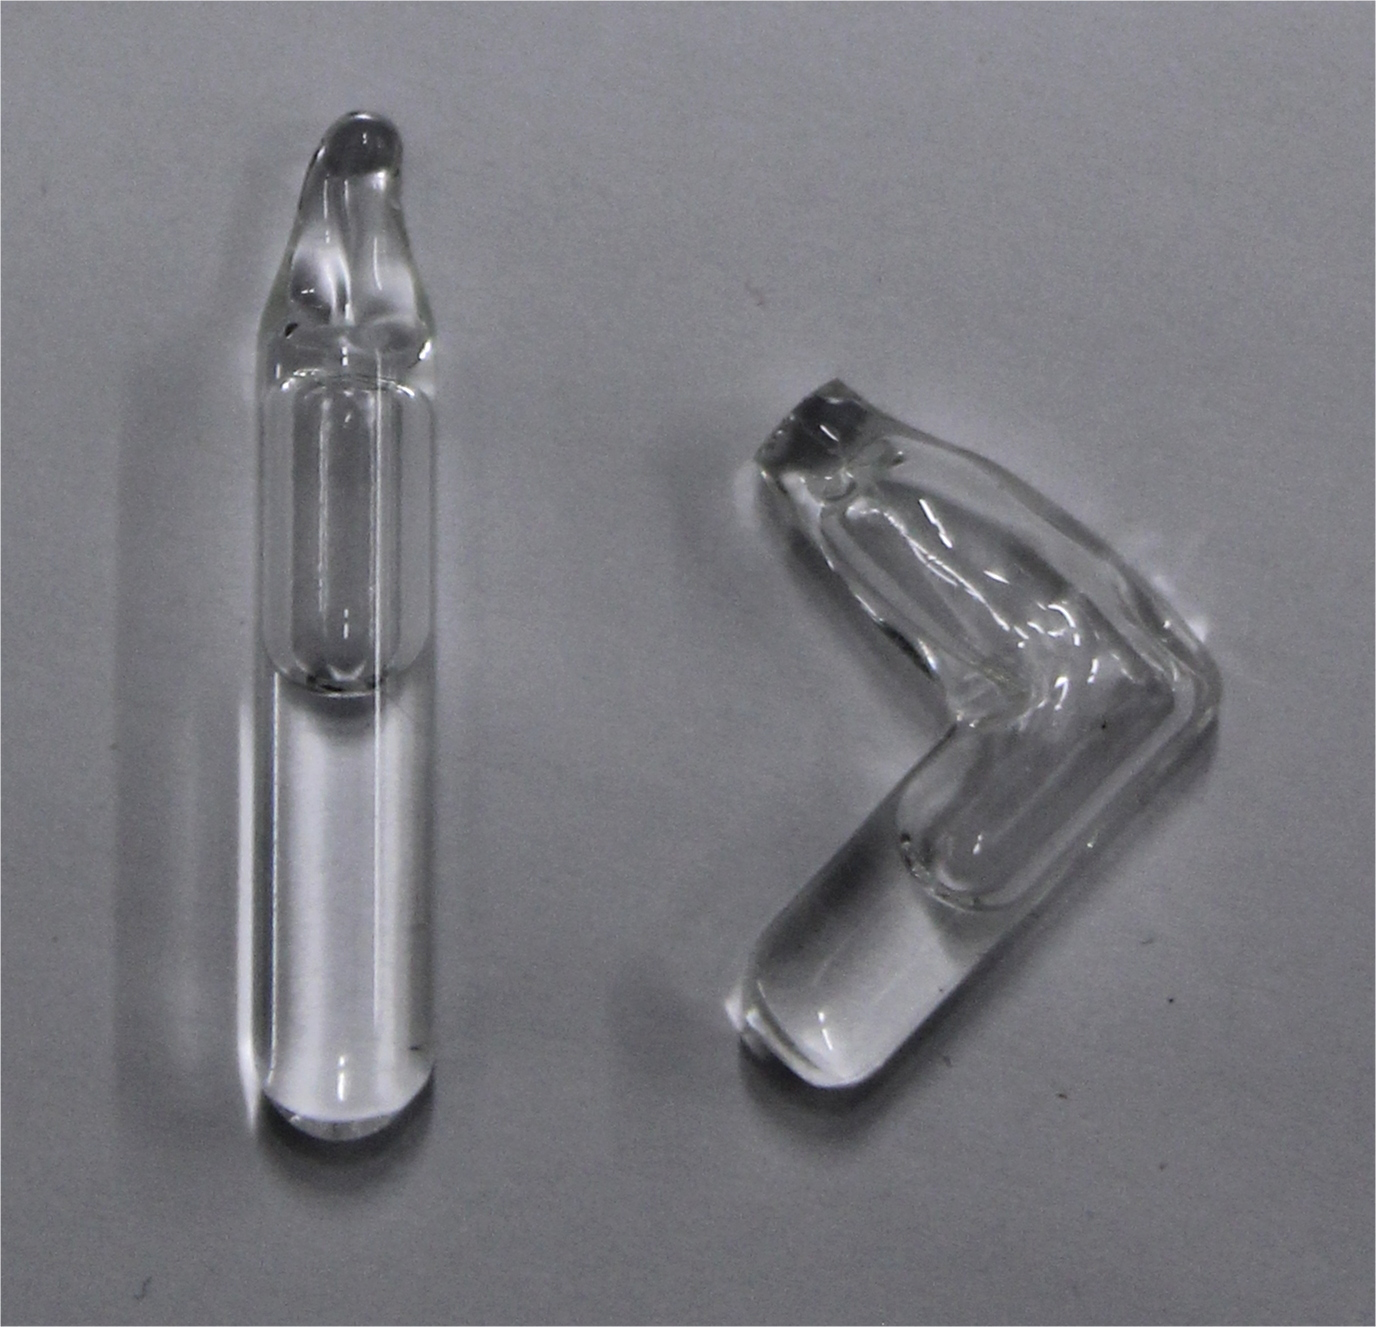
\includegraphics[width=\textwidth]{graphics/proben/RbCl_in_D20.jpg}
		\caption{ }
		\label{fig:exp:probe_d}
	\end{subfigure}
	\caption{Fotografien der verwendeten Proben. Die Merkmale finden sich in Tabelle \ref{tab:exp:proben}}
	\label{fig:exp:proben}
\end{figure}

Die Herstellung von C. Zürns Probe 1 ist in \cite{zuern_arbeit} dokumentiert. Der Herstellungsprozess gleich im Wesentlichen dem im Folgenden beschriebenen.

Für die Herstellung der Proben 3 und 4 wurde Calciumrubidiumnitrat zu einem möglichst feinen Pulver zermörsert und ein gerades bzw. gebogenes Duran-Glas-Röhrchen gefüllt. Um störende Einflüsse von Feuchtigkeit in der Probe möglichst gut zu elimieren, wurden die Proben dann über Nacht bei $\SI{160}{\degreeCelsius}$ in einem evakuierten Ofen getrocknet, der im Anschluss mit Stickstoffgas gelöscht wurde.

So präpariert wurden die Proben unter Anwendung eines Freeze-Pump-Thaw-Ver\-fah\-rens von einem Glasbläser der TU Dortmund, abgeschmolzen. Mit dem Verfahren soll der Probe möglichst viel Gas entzogen werden, indem sie Vakuum ausgesetzt wird. Damit die Probe aber nicht mit angesaugt wird, wird sie vor dem Abpumpen eingefroren und danach wieder getaut. Nach dem Abschmelzen wurden die Proben durch Erhitzen geschmolzen, um sie dann in einem Glaszustand abkühlen zu lassen.

Mit dem gleichen Verfahren wurde am 13.07.2017 die Probe 2 erstellt, wobei hier die Probe \emph{vor} dem Abschmelzen in den Glaszustand gebracht wurde. Tests mit dieser Probe zeigten jedoch, dass sie kaum stabil im Glaszustand zu halten war sondern schnell auskristallisierte.

Zum Bestimmen der Larmorfrequenz von $^\text{87}$Rb wurden zudem zwei Proben, Proben 5 und 6, mit in D$_\text{2}$O gelöstem RbCl erstellt. Es wurde eine gesättigte Lösung mit etwas weniger als $\SI{1}{mg}$ RbCl pro $\SI{1}{ml}$ D$_\text{2}$O erstellt, welche in Duran-Glas-Röhrchen eingefüllt wurde. Um die Proben unter Vakuum abschmelzen zu können, mussten sie zuerst gefroren werden. Dazu wurden die Spitzen der Proben in flüssigen Stickstoff getaucht, sodass die sich in Spitze befindliche Lösung gefriert, der Rest der Probe jedoch zunächst flüssig bleibt. Dies gibt dem, durch den Übergang zum Eis gestiegenen Volumen, Raum zum Ausweichen, was ein Springen des Glasröhrchens verhindern soll. Anschließend wurden die Proben durch Eintauchen in flüssigen Stickstoff komplett eingefroren und dann abgeschmolzen. An den verwendeten Spektrometern wurde die Larmorfrequenz für $^\text{87}$Rb jedoch schon zuvor auf $\omega_{L, \text{OBI}} = 2\pi \cdot \SI{97.1722}{MHz}$ und $\omega_{L, \text{Bruker}} = 2\pi \cdot \SI{130.9736}{MHz}$ bestimmt, sodass diese Proben an diesen Spektrometern nicht verwendet werden mussten.

In dieser Arbeit wurden die Proben 1 und 4 verwendet. Mit dem OBI-Spektrometer wurde ausschließlich Probe 1 verwendet, mit dem Bruker-Spektrometer ausschließlich Probe 4.

Probe 1 wurde schon in der Arbeit \cite{joachim_master} verwendet. Hier traten Probleme mit einem häufigen Auskristallisieren der Probe auf. Dieses Problem trat Verlauf der Arbeit nur sehr selten auf, sodass ein größerer Temperaturbereich abgedeckt werden konnte. Wodurch diese Änderung bewirkt wurde, ist nicht bekannt.
